\begin{figure}[htbp]\centering
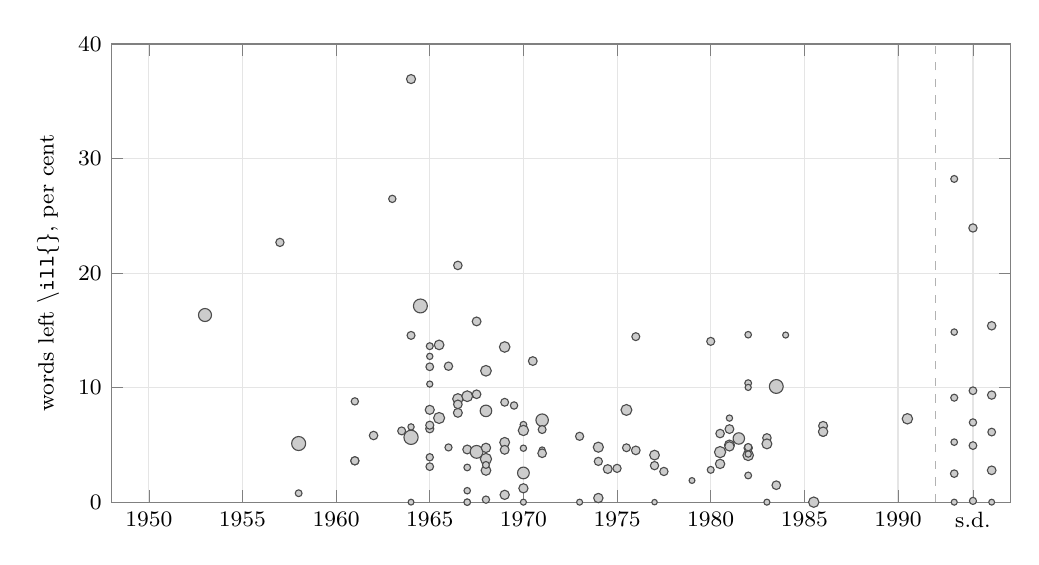
\begin{tikzpicture}
\begin{axis}[width=13cm,height=7.4cm,xmin=1948,xmax=1996,ymin=0,ymax=40,
  xtick={1950,1955,1960,1965,1970,1975,1980,1985,1990,1994},xticklabels={1950,1955,1960,1965,1970,1975,1980,1985,1990,s.d.},
  ylabel={words left \texttt{\textbackslash ill\{\}}, per cent},grid=major,grid style={black!10},
  tick label style={font=\footnotesize},label style={font=\footnotesize},axis line style={black!50}]
\draw[black!30,dashed] (axis cs:1992,0) -- (axis cs:1992,40);
\addplot[scatter,only marks,mark=*,scatter/use mapped color={draw=black!70,fill=black!20},
  visualization depends on={\thisrow{p} \as \p},scatter/@pre marker code/.append style={/tikz/mark size={0.8pt+0.13pt*sqrt(\p)}},
  point meta=\thisrow{p}] table[x=y,y=u] {
y u p
1953 16.34 142
1957 22.68 28
1958 0.78 11
1967 4.60 38
1968 2.77 54
1966.5 9.02 69
1969 5.22 57
1969 8.72 23
1958 5.12 178
1961 3.61 27
1967.5 4.39 136
1965 8.06 42
1968 3.77 90
1971 7.16 124
1966.5 7.80 39
1970.5 12.32 36
1965.5 7.35 85
1963.5 6.22 24
1965 11.82 21
1967 9.25 78
1967 1.00 8
1966 11.87 30
1970 6.76 10
1964 5.66 186
1968 11.47 76
1970 1.21 44
1970 0.00 5
1970 6.26 67
1965 3.92 16
1965 6.41 27
1965 13.62 12
1965 10.31 6
1964.5 17.13 174
1964 6.57 7
1965.5 13.73 53
1969 13.55 73
1967 0.00 5
1965 12.73 7
1973 5.75 27
1971 4.56 5
1961 8.80 16
1962 5.82 32
1964 36.94 42
1965 6.72 26
1966.5 8.54 34
1963 26.48 16
1964 0.00 4
1980.5 4.37 90
1980.5 3.34 47
1976 4.52 35
1976 14.45 24
1977.5 2.68 29
1977 4.11 54
1981 4.99 59
1981 4.87 46
1982 4.09 73
1977 3.19 29
1964 14.56 24
1965 3.10 20
1966 4.78 14
1966.5 20.67 32
1967.5 9.42 34
1967.5 15.78 37
1967 3.03 10
1974 0.42 16
1982 4.73 30
1982 10.39 11
1982 4.80 16
1973 0.00 5
1983.5 1.48 34
1968 0.22 16
1982 4.20 7
1983 0.00 5
1982 2.33 11
1981 7.34 7
1983 5.15 16
1983 5.61 32
1975.5 4.75 23
1974 4.80 63
1969.5 8.44 17
1969 4.57 38
1970 4.71 7
1970 2.55 103
1971 4.27 34
1971 6.34 24
1974 3.56 27
1974.5 2.89 38
1979 1.89 4
1974 0.36 47
1975.5 8.05 81
1977 0.00 2
1980 14.04 25
1980 2.82 12
1980.5 5.99 32
1981 6.38 37
1983 5.09 59
1981.5 5.56 95
1985.5 0.00 68
1982 14.62 9
1982 10.02 6
1983.5 10.10 171
1984 14.59 5
1986 6.18 26
1986 6.07 18
1986 6.66 40
1986 6.15 48
1990.5 7.28 69
1968 7.97 98
1968 4.74 47
1961 3.61 28
1968 3.25 12
1975 2.95 27
1967 0.00 9
1969 0.64 45
1993 28.22 12
1994 23.94 29
1995 15.40 31
1993 14.85 8
1994 9.73 21
1995 9.35 30
1993 9.12 13
1994 6.96 16
1995 6.12 21
1993 5.24 9
1994 4.94 21
1995 2.78 35
1993 2.49 19
1994 0.11 14
1995 0.00 4
1993 0.00 5
};
\end{axis}
\end{tikzpicture}
\caption{The share of words the first pass could not read, folder by folder, against the middle of the inventory's dating; 16 undated folders stand in the column at the right. A larger dot, more pages transcribed. 130 folders, 505,415 words read and 39,397 left illegible (7.2 per cent). No trend is drawn: the datings are ranges, often decades wide. The count is of the apparatus, not of the ink. From \texttt{src/content/hand.json} (2026-09-26), after the site's page \emph{The hand}.}\label{fig:hand}
\end{figure}
